% Fichier  : projet.tex
% Format   : LaTeX file
% Auteur   : Florent Hivert
% A propos : Master 2 / Combinatoire
% Date     : lun. oct.  2 14:09:41 CEST 2017
%%%%%%%%%%%%%%%%%%%%%%%%%%%%%%%%%%%%%%%%%%%%%%%%%%%%%%%%%%%%%%%%%%%%%%%%%%%%%%%
\documentclass[11pt]{article}
\usepackage{styles/tdtp,array,amsmath}
\usepackage[T1]{fontenc}
\usepackage[utf8]{inputenc}
\usepackage[francais]{babel}
\usepackage{multicol}
\usepackage{styles/tikz-uml}

\newcommand\todo[1]{\textcolor{red}{ToDo: #1}}

\usetikzlibrary{positioning}
%
%\CORRECTIONtrue
\projet{de Combinatoire}
\course{Master d'informatique}
\group{Génération Combinatoire}
\theme{Génération d'objets combinatoires décrit par une grammaire}
%
\newcommand{\cpl}[1]{\overline{#1}}
\renewcommand{\emph}[1]{\textbf{#1}}
\newcounter{asuivre}
\newenvironment{ask}{\begin{enumerate}}%
                       {\setcounter{asuivre}{\theenumi}\end{enumerate}}
\newenvironment{asks}{\begin{enumerate}\setcounter{enumi}{\theasuivre}}%
                       {\setcounter{asuivre}{\theenumi}\end{enumerate}}


\newcommand{\Python}{\texttt{Python}}

\begin{document}
\maketitle

\begin{abstract}
  Le but de ce projet est de compter et d'engendrer l'ensemble des objets
  combinatoires décrits par une grammaire. Il est ainsi possible d'engendrer
  une grande variété d'objets comme des arbres ou des mots.  \smallskip

  Le projet sera implanté en \Python{}. On pourra travailler seul ou en
  binôme. La date de remise sera précisée ultérieurement. Toutes les fonctions
  de ce projet devront être commentées et testées.

  On rédigera également un \textbf{rapport} présentant les fonctionnalités et
  répondant aux questions théoriques du sujet. Les algorithmes et choix
  d'implantations devront être expliqués. 
\end{abstract}

\section{Introduction : quelques exemples}
%%%%%%%%%%%%%%%%%%


\subsection{Les arbres binaires complets}

Un \emph{arbre binaire complet} est soit une feuille, soit un noeud sur lequel
on a greffé deux arbres binaires complets. Dans la suite de ce sujet, on
suppose les arbres déjà implanté avec un constructeur \texttt{Node(l, r)} pour
les noeuds et une constante \texttt{Leaf} pour les feuilles. Pour votre
projet, vous pouvez reprendre ce que vous avez écrit en TP.
\begin{verbatim}
   >>> tr = Node(Leaf, Node(Leaf, Leaf))
\end{verbatim}
On peut ainsi décrire l'ensemble des arbres binaires par les définitions
récursives suivantes:
\begin{itemize}
\item l'ensemble \texttt{"Trees"} des arbres est la réunion disjointe (que
  l'on notera en \Python{} par le constructeur \texttt{UnionRule}) de deux
  ensembles : l'ensemble \texttt{"Nodes"} des noeuds et l'ensemble
  \texttt{"Leaf"} des feuilles;
\item l'ensemble \texttt{"Nodes"} des noeuds est obtenu à partir de l'ensemble
  des paires d'arbres, c'est-à-dire le produit cartésien (noté par le
  constructeur \texttt{ProdRule}) de l'ensemble des arbres avec lui même;
\item il n'y a qu'un seul arbre possible constitué d'une feuille. C'est le
  singleton (constructeur \texttt{SingletonRule}) \texttt{"Leaf"}.
\end{itemize}
Une telle définition est appelée \emph{grammaire}. On écrira en
\Python\ la grammaire des arbres de la manière suivante:
\begin{verbatim}
    treeGram = {"Tree" : UnionRule("Node", "Leaf"),
                "Node" : ProductRule("Tree", "Tree", 
                                     lambda (a, b) : Node(a, b)),
                "Leaf" : SingletonRule(Leaf)}
    init_grammar(treeGram)
\end{verbatim}
Le but de ce projet est d'implanter un algorithme permettant de compter,
d'engendrer automatiquement la liste ainsi que de tirer au hasard un des
objets décrit par une grammaire de ce type : par exemple il y a 5 arbres
binaires complets à quatre feuilles:
\begin{center}
  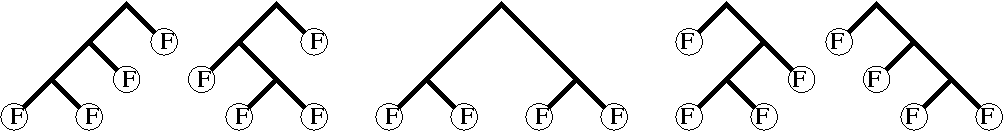
\includegraphics[width=10cm]{arbres.pdf}
\end{center}


\noindent Ce que l'on peut obtenir par le programme
\begin{verbatim}
    >>> treeGram['Tree'].count(4)
    5
\end{verbatim}
La liste des objets décrits par la grammaire peut ensuite être obtenue comme
suit:
\begin{verbatim}
    >>> for t in treeGram['Tree'].list(4): print t
    Node(Leaf, Node(Leaf, Node(Leaf, Leaf)))
    Node(Leaf, Node(Node(Leaf, Leaf), Leaf))
    Node(Node(Leaf, Leaf), Node(Leaf, Leaf))
    Node(Node(Leaf, Node(Leaf, Leaf)), Leaf)
    Node(Node(Node(Leaf, Leaf), Leaf), Leaf)
\end{verbatim}


\subsection{Les mots de Fibonacci}

On appelle mot de Fibonacci tout mot sur l'alphabet \texttt{A} et \texttt{B}
qui ne contient pas deux \texttt{B} à la suite. Un tel mot $w$ est décrit par
la grammaire suivante:
\begin{itemize}
\item soit $w$ est vide;
\item soit $w$ est de la forme $\texttt{A} u$ où $u$ est un mot de Fibonacci;
\item soit $w$ est le mot $\texttt{B}$;
\item soit $w$ est de la forme $\texttt{B} \texttt{A} u$ où $u$ est un mot de Fibonacci;
\end{itemize}
Ceci ce traduit en \Python\ par la grammaire:
\begin{verbatim}
    fiboGram = {"Fib"    : UnionRule("Vide", "Cas1"),
                "Cas1"   : UnionRule("CasAu", "Cas2"),
                "Cas2"   : UnionRule("AtomB", "CasBAu"),
                "Vide"   : EpsilonRule(""),
                "CasAu"  : ProductRule("AtomA", "Fib", "".join),
                "AtomA"  : SingletonRule("A"),
                "AtomB"  : SingletonRule("B"),
                "CasBAu" : ProductRule("AtomB", "CasAu", "".join)}
    init_grammar(fiboGram)
\end{verbatim}
Note: La commande \verb+"".join+ utilise la méthode \texttt{join} de la classe
\texttt{string} qui concatène une liste ou un tuple de chaînes de caractères
passé en argument:
\begin{verbatim}
    >>> "".join(["ab","toto"])
    'abtoto'
\end{verbatim}
Voici la liste des mots de Fibonacci de longueur 3: \texttt{AAA},
\texttt{AAB}, \texttt{ABA}, \texttt{BAA}, \texttt{BAB}.  Ce qui se calcule en
\Python{} par
\begin{verbatim}
    >>> fiboGram['Fib'].count(3)
    5
    >>> fiboGram['Fib'].list(3)
    ['AAA', 'AAB', 'ABA', 'BAA', 'BAB']
\end{verbatim}
On peut de la même manière obtenir les 21~mots de Fibonacci de longueur~6:
\begin{verbatim}
    >>> fiboGram['Fib'].list(6)
    ['AAAAAA', 'AAAAAB', 'AAAABA', 'AAABAA', 'AAABAB', 'AABAAA', 'AABAAB', 
     'AABABA', 'ABAAAA', 'ABAAAB', 'ABAABA', 'ABABAA', 'ABABAB', 'BAAAAA', 
     'BAAAAB', 'BAAABA', 'BAABAA', 'BAABAB', 'BABAAA', 'BABAAB', 'BABABA']
\end{verbatim}




\section{Définitions formelles}
%%%%%%%%%%%%%%%%%%%%%%%%%%%%%%%%%%%%%%

Une grammaire décrit récursivement un ensemble d'objets. Elle est constituée
d'un ensemble de règles ayant chacune un nom (chaîne de caractères). Le nom
d'une règle est appelé \emph{symbole non-terminal} ou plus simplement
non-terminal de la grammaire.  \medskip

Une \emph{règle de grammaire} $R$ décrit un ensemble qui est
\begin{itemize}
\item[$\bullet$] soit un singleton dont le seul élément est un objet
  \emph{atomique} et qui sera de poids 1 (par exemple la feuille d'un arbre).
\item[$\bullet$] soit un ensemble dont le seul élément est un objet
  \emph{vide} qui sera de poids 0 (par exemple la chaîne vide).
\item[$\bullet$] soit l'\emph{union de deux ensembles} décrit par deux
  non-terminaux $N_1$ et $N_2$;
\item[$\bullet$] soit en bijection avec le \emph{produit cartésien de deux
    ensembles} décrit par deux non-terminaux $N_1$ et $N_2$; L'ensemble est
  alors construit à partir des paires d'éléments $(e_1, e_2) \in N_1 \times
  N_2$. Dans ce cas, il faut de plus donner à \Python\ la bijection qui
  construit l'objet correspondant à la paire $(e_1, e_2)$ (concaténation pour
  les chaînes de caractères où constructeur \texttt{Node} pour les arbres).
\end{itemize}
\medskip

La \emph{taille} ou \emph{poids} d'un objet est le nombre d'atomes qu'il
contient. Le poids d'un élément correspondant à une paire $(e_1, e_2)$ est
donc la somme des poids de $e_1$ et de $e_2$.

À chaque non-terminal on associe la taille du plus petit objet qui en dérive.
Cette taille est appelé \emph{valuation} du non-terminal.


\subsection{Structures de données}

On modélise chacune de ces classes combinatoires décrites récursivement par un
objet (au sens de la programmation orientées objets) \Python. Dans l'exemple
des arbres binaires, l'objet \verb+treeGram["Tree"]+ modélise l'ensemble de
tous les arbres binaires. Cet ensemble est construit comme l'union de deux
sous ensembles modélisés par les objets \verb+treeGram["Node"]+ et
\verb+treeGram["Leaf"]+.  La classe de l'objet \verb+treeGram["Tree"]+ est
ainsi \verb+UnionRule+, il est construit grâce à un appel au constructeur par
\verb+UnionRule("Node", "Leaf")+.


Une grammaire sera stockée sous la forme d'un dictionnaire qui associe un
objet à une chaîne de caractère. Dans le but de ne pas recopier plusieurs fois
du code, on utilisera avantageusement la programmation objet et
l'héritage. Ainsi chaque règle de grammaire sera un objet de la classe
abstraite \texttt{AbstractRule}. On distingue deux types de règles de
grammaires:\smallskip

\begin{itemize}
\item les règles de constructions qui sont les objets des classes
  \texttt{UnionRule} et \texttt{ProductRule} qui dérivent de la classe abstraite
  \texttt{ConstructorRule};\smallskip

\item les règles de constantes qui sont les objets des classes
  \texttt{SingletonRule} et \texttt{EpsilonRule} qui dérivent de la classe abstraite
  \texttt{ConstantRule};
\end{itemize}
\bigskip

Voici un schéma de la
hiérarchie de classe: \bigskip

\begin{center}
\begin{tikzpicture}
\umlclass[y=3.5]{AbstractRule}{
  \_grammar : dict
}{
  \_set\_grammar(gram)}
\umlclass[x=-4,y=0]{ConstructorRule}{
  \_parameters : tuple\\
  \_valuation : int
}{
  valuation() : int\\
  \_update\_valuation()
}
\umlclass[x=4,y=0]{ConstantRule}{
  \_object : object\\
}{
  valuation() : int\\
}
\umlclass[x=-6,y=-4]{UnionRule}{
%  \_left\_right : fun
}{
  \_calc\_valuation()\\
}
\umlclass[x=-2,y=-4]{ProductRule}{
  \_constructor : fun\\
%  \_right : fun\\
%  \_left : fun
}{
  \_calc\_valuation()\\
}
\umlclass[x=2,y=-4]{SingletonRule}{}{}
\umlclass[x=6,y=-4]{EpsilonRule}{}{}

\umlinherit{ConstructorRule}{AbstractRule}
\umlinherit{ConstantRule}{AbstractRule}
\umlinherit{ProductRule}{ConstructorRule}
\umlinherit{UnionRule}{ConstructorRule}
\umlinherit{SingletonRule}{ConstantRule}
\umlinherit{EpsilonRule}{ConstantRule}
\end{tikzpicture}
\end{center}
\smallskip

Voici la liste des  constructeurs (méthodes \verb+__init__+) des différentes
classes avec les paramètres et leurs types:
\begin{itemize}
\item[$\bullet$] \verb+SingletonRule.__init__(self, obj)+ où \texttt{obj} est
  un \texttt{object} python quelconque;
\item[$\bullet$] \verb+EpsilonRule.__init__(self, obj)+ où \texttt{obj} est un
  \texttt{object} python quelconque.
\item[$\bullet$] \verb+UnionRule.__init__(self, fst, snd)+ où \texttt{fst} et
  \texttt{snd} sont deux non terminaux (de type \Python{} \texttt{string});
\item[$\bullet$] \verb+ProductRule.__init__(self, fst, snd, cons)+ où
  \texttt{fst} et \texttt{snd} sont deux non terminaux et \texttt{cons} est
  une fonction qui prend un couple d'\texttt{object} et qui retourne un
  \texttt{object}.
\end{itemize}
\bigskip

En plus des méthodes listées dans ce diagramme, chaque classe devra implanter
(ou bien hériter) les méthodes d'énumération suivantes: \texttt{count, list, unrank, random},\dots

\medskip

Le principal problème d'implantation provient du fait qu'une grammaire est un
\emph{ensemble de définitions mutuellement récursives}. Il y a donc un travail
à faire pour «~casser des boucles infinies~» et s'assurer que la récursion est
bien fondée. Voici quelques éléments permettant de résoudre ce problème:
\begin{itemize}
\item Pour les règles constructeur par exemple
  \verb+UnionRule("Node", "Leaf")+ les sous règles (ici: \verb+"Node"+ et
  \verb+"Leaf"+) ne sont connues que par les chaînes de caractères qui
  représentent les symboles non terminaux. Pour pouvoir associer ces chaînes
  aux objets associés, il faut que l'objet \verb+UnionRule("Node", "Leaf")+
  ait accès à la grammaire.
\item Au moment de la construction d'une règle, la grammaire qui va contenir
  la règle n'existe pas encore; il faut donc attendre que la grammaire soit
  complètement créée pour appeler la méthode \texttt{\_set\_grammar} sur
  chaque règle. C'est le rôle de la fonction \texttt{init\_grammar}.
\item La fonction \texttt{init\_grammar} se charge également de calculer les
  valuations selon l'algorithme décrit plus bas.
\end{itemize}
\medskip

\subsection{A rendre sur papier}

\begin{ask}
\item Pour les grammaires des arbres et des mots de Fibonnacci, donner dans un
  tableau pour $n=0,\dots,10$ les réponses attendue pour la méthode
  \texttt{count} pour les $8$ non terminaux des mots de Fibonnacci et les 3 non terminaux des arbres binaires,
\item Donner la grammaire de tous les mots sur l'alphabet \texttt{A,B}.
\item Donner la grammaire des mots de Dyck, c'est-à-dire les mots sur
  l'alphabet $\{\texttt{(}, \texttt{)}\}$ et qui sont correctement
  parenthésés.
\item Donner la grammaire de mots sur l'alphabet \texttt{A,B} qui n'ont pas
  trois lettres consécutivement égales.
\item Donner la grammaire des palindromes sur l'alphabet \texttt{A},
  \texttt{B}, même question sur l'alphabet \texttt{A,B,C}.
\item Donner la grammaire des mots sur l'alphabet \texttt{A,B} qui
  contiennent autant de lettres \texttt{A} que de lettres \texttt{B}.
\end{ask}

\begin{asks}
\item Écrire une fonction qui vérifie qu'une grammaire est correcte,
  c'est-à-dire que chaque non-terminal apparaissant dans une règle est bien
  défini par la grammaire.
\end{asks}



\section{Algorithmes}
%%%%%%%%%%%%%%%%%%%%%%%%%%%%%%%%%%%%%%

On demande d'implanter les algorithmes de calculs suivants (dans ce qui suit
\texttt{rule} est une règle quelconque):
\begin{itemize}
\item Calcul de la valuation d'une grammaire (ce qui permet de vérifier la
  grammaire);
\item méthode \verb+rule.count(self, n)+ qui calcule le nombre d'objets d'un
  poids donné $n$ par la méthode naïve;
\item méthode \verb+rule.list(self, n)+ qui calcule la liste des objets de poids
  $n$;
\item méthode \verb+rule.unrank(self, n, i)+ qui calcule le $i$-ème élément de
  la liste des objets de poids $n$, sans calculer la liste; Note importante:
  en \Python{} la position dans une liste commence à $0$;
\item méthode \verb+rule.random(self, n)+ qui choisit équitablement au hasard
  un objet de poids $n$ (on utilisera \verb+rule.unrank(self, n, i)+ où $i$
  sera choisi aléatoirement).
\end{itemize}

Le calcul de la valuation est nécessaire aux étapes suivantes qui sont
indépendantes. Je les ai néanmoins classé par ordre croissant de difficulté.

\subsection{Calcul de la valuation}

La \emph{valuation} du non-terminal \texttt{nt} est la taille du plus petit
objet qui en dérive. La valuation d'une grammaire est l'ensemble des
valuations des terminaux. Elle vérifie les quatres règles suivantes:
\begin{itemize}
\item[$\bullet$] la valuation d'un \texttt{Singleton} est 1;
\item[$\bullet$] la valuation d'un \texttt{Epsilon} est 0;
\item[$\bullet$] la valuation de l'union \texttt{Union} des non-terminaux
  $N_1$ et $N_2$ est le minimum des valuations de $N_1$ et de $N_2$;
\item[$\bullet$] la valuation du produit \texttt{Prod} des non-terminaux $N_1$
  et $N_2$ est la somme des valuations de $N_1$ et de $N_2$;
\end{itemize}

Pour la calculer, on utilise l'algorithme de point fixe suivant. On part de la
valuation $V_0$ (incorrecte) qui associe à chaque non-terminal la valeur
$\infty$. En appliquant une fois non récursivement (pour éviter les boucles
infinies) les règles précédentes à partir de $V_0$, on calcule une nouvelle
valuation $V_1$.  On calcule ensuite de même une valuation $V_2$ a partir de
$V_1$. On recommence tant que la valuation $V_n$ est différente de
$V_{n-1}$. La valuation cherchée $V := V_n$ est obtenue quand $V_n=V_{n-1}$.
\bigskip

\noindent\textbf{Note:} Si $V(N) := V_n(N) = \infty$ pour un certain non terminal
$N$, alors aucun objet ne dérive de ce non-terminal. On considère alors que la
grammaire est incorrecte.  \bigskip

Par exemple, sur les arbres, le calcul se fait en $4$ étapes:
$$\begin{array}{|c|ccc|}
\hline
  n     &  \texttt{Tree}  &  \texttt{Leaf}  &  \texttt{Node} \\
\hline\hline
  \text{règle:} & \min(V_{n-1}(\texttt{Leaf}),V_{n-1}(\texttt{Node}))
               & 1
               & V_{n-1}(\texttt{Tree}) + V_{n-1}(\texttt{Tree}) \\
\hline\hline
  0     &  \infty         &  \infty         &  \infty        \\
  1     &  \infty         &  1              &  \infty        \\
  2     &  1              &  1              &  \infty        \\
  3     &  1              &  1              &  2             \\
  4     &  1              &  1              &  2             \\
\hline
 \text{Final} &  1              &  1              &  2             \\
\hline
\end{array}$$

\subsubsection{À faire:}

\begin{asks}
\item À rendre sur papier: Pour les différentes grammaire considérée, appliquer
  l'algorithme à la main et donner les valuations des différents non
  terminaux.
\item Écrire un fonction \texttt{init\_grammar} qui prend en paramètre une
  grammaire, qui appelle sur chaque règle de la grammaire la méthode
  \verb+set_grammar+ et qui implante l'algorithme de calcul de la valuation. 
\end{asks}

\subsection{Comptage naïf du nombre d'objets}

Le comptage du nombre d'objets de poids $i$ se fait en appliquant
récursivement les règles suivantes:
Soit $N$ un non-terminal. On note $C_N(i)$ le nombre d'objet de poids $i$.
\begin{itemize}
\item[$\bullet$] si $N$ est un \texttt{Singleton} alors $C_N(1) = 1$ et $C_N(i)
  = 0$ si $i$ est différent de $1$;
\item[$\bullet$] si $N$ est un \texttt{Epsilon} alors alors $C_N(0) = 1$ et
  $C_N(i) = 0$ si $i$ est différent de $0$;
\item[$\bullet$] si $N$ est l'union \texttt{Union} des non-terminaux $N_1$ et
  $N_2$ alors
  $$C_N(i) = C_{N_1}(i) + C_{N_2}(i)\,;$$
\item[$\bullet$] si $N$ est le produit \texttt{Prod} des non-terminaux $N_1$ et
  $N_2$
  $$C_N(i) = \sum_{k+l=i} C_{N_1}(k) \cdot C_{N_2}(l)\,;$$
  \emph{Pour aller plus
    vite et éviter des boucles infinies}, on ne considérera dans la somme
  précédente que les cas où $k \geq V(N_1)$ et $l \geq V(N_2)$, où $V(N)$
  désigne la valuation du non-terminal $N$. En effet, par définition
  $C_N(i) = 0$ si $V(N) > i$. 
\end{itemize}

\subsubsection{À faire:}
\begin{asks}
\item Implanter pour chaque règle de grammaire une méthode
  \texttt{count} qui compte le nombre d'objets d'une grammaire dérivant
  d'un non-terminal et d'un poids donné.
\end{asks}


\subsection{Calcul de la liste des objets}

On applique récursivement les définitions des constructeurs
\texttt{Singleton}, \texttt{Epsilon}, \texttt{Union} et \texttt{Prod} pour
construire la liste des objets de taille $i$. En particulier, si $N$ est le
produit \texttt{Prod} des non-terminaux $N_1$ et $N_2$, la liste des objets
dérivant de $N$ et de poids $i$ est la concaténation des listes de tous les
produits cartésiens d'éléments dérivant de $N_1$ et de taille $k$ et
d'éléments dérivant de $N_2$ et de taille $l$, pour tous les couples $k,l$
tels que $k+l=i$, $k \geq V(N_1)$ et $l \geq V(N_2)$ (comme précédemment
$V(M)$ désigne la valuation du non-terminal $M$).

Par exemple, pour obtenir les arbres de taille $3$, on procède de la manière
suivante

\noindent Calcul de \texttt{Tree = Union (Leaf, Node)} avec $i=3$.
\begin{itemize}
\item Application de \texttt{Leaf = Singleton Leaf} avec $i=3$, on retourne
  la liste vide \texttt{[]};
\item Application de \texttt{Node = Prod(Tree, Tree)} avec $i=3$. La valuation
  de \texttt{Tree} est 1. Il y a donc deux possibilités $3=1+2$ ou $3=2+1$.
  \begin{enumerate}
  \item \begin{itemize}  
    \item Application de \texttt{Tree = Union (Leaf, Node)} avec $i=2$.
      \begin{itemize}
      \item \texttt{Leaf} est vide avec $i=2$ on retourne la liste vide.
      \item Application de \texttt{Node = Prod(Tree, Tree)} avec $i=2$. La
        valuation de \texttt{Tree} est 1. Une seule décomposition est possible
        $1+1$\dots\ On appelle donc deux fois \texttt{Tree} avec $i=1$\dots\ 
        (Je n'écrit pas les appels récursifs)\dots\ qui retourne la liste
        \texttt{[Leaf]}. On retourne donc la liste
        $$\texttt{[Node(Leaf, Leaf)]}$$
      \end{itemize}
    \item Application de \texttt{Tree = Union (Leaf, Node)} avec $i=1$.
      On retourne la liste 
        $$\texttt{[Leaf]}$$
    \end{itemize}
    Le produit cartésien des deux listes précédentes est la liste formée du
    seul élément
    $$\texttt{[Node(Node(Leaf, Leaf), Leaf)]}$$
  \item \begin{itemize}  
    \item Application de \texttt{Tree = Union (Leaf, Node)} avec $i=1$.
      On retourne donc la liste
      $$\texttt{[Leaf]}$$
    \item Application de \texttt{Tree = Union (Leaf, Node)} avec $i=2$.
      On retourne donc la liste
      $$\texttt{[Node(Leaf, Leaf)]}$$
    \end{itemize}
    Le produit cartésien des deux listes précédentes est la liste formée du
    seul élément
    $$\texttt{[Node(Leaf, Node(Leaf, Leaf))]}$$
  \end{enumerate}
  On retourne donc la liste des deux arbres:
\begin{verbatim}

[Node(Leaf, Node(Leaf, Leaf)), Node(Node(Leaf, Leaf), Leaf)]

\end{verbatim}
\end{itemize}
\bigskip

Pour $i=6$, il faut essayer les décompositions $6=5+1$, $6=4+2$, $6=3+3$,
$6=2+4$ et $6=1+5$. Étudions le cas $3+3$. Par appel récursif on trouve deux
arbres de poids $3$:
\begin{verbatim}
 [Node(Node(Leaf, Leaf), Leaf); Node(Leaf, Node(Leaf, Leaf))]
\end{verbatim}
Le produit cartésien est donc formé de $4$ éléments qui correspondent aux $4$
arbres suivants:
\begin{verbatim}
 Node(Node(Leaf, Node(Leaf, Leaf)), Node(Node(Leaf, Leaf), Leaf));
 Node(Node(Node(Leaf, Leaf), Leaf), Node(Node(Leaf, Leaf), Leaf));
 Node(Node(Leaf, Node(Leaf, Leaf)), Node(Leaf, Node(Leaf, Leaf)));
 Node(Node(Node(Leaf, Leaf), Leaf), Node(Leaf, Node(Leaf, Leaf)));
\end{verbatim}


\subsection{Calcul du $i$-ème élément : la méthode \texttt{unrank}}

Pour calculer l'élément de taille $n$ et de rang $i$, on fait appel à la
méthode \texttt{unrank}. Voici par exemple l'arbre de taille $6$ et de rang
$12$.
\begin{verbatim}
    >>> treeGram['Tree'].unrank(6, 12)
    Node(Leaf, Node(Node(Node(Leaf, Node(Leaf, Leaf)), Leaf), Leaf))
\end{verbatim}
\textbf{Attention ! La numérotation commence à zéro.}

On procédera récursivement comme suit:
\begin{itemize}
\item si l'on demande un objet dont le rang est supérieur au nombre d'objet on
  lève une exception \texttt{ValueError}.
\item dans le cas \texttt{EpsilonRule} ou \texttt{SingletonRule}, on retourne
  l'objet.
\item dans le cas d'une union: \texttt{"U" : UnionRule("A", "B")}, on suppose
  connu les nombres d'objets: $C_U(n) = C_A(n) + C_B(n)$. Alors l'objet de $U$
  de rang $i$ est l'objet de $A$ de rang $i$ si $i<C_A(n)$ et l'objet de $B$
  de rang $i-C_A(n)$ sinon.
\item dans le cas d'un produit: \texttt{"U" : ProductRule("A", "B")}, on suppose
  connu les nombres d'objets:
  $$
  C_U(n) = \sum_{i=0}^n C_A(i)\,C_B(n-i)\,.
  $$
  En s'inspirant de l'union, on calcule la valeur de $i$:
  $$
  U(n) = \bigsqcup_{i=0}^n A(i) \times B(n-i)\,.
  $$
  Il reste finalement à trouver l'élément de rang $j$ d'un produit cartésien
  d'ensemble $A\times B$ où $A=\{a_1,\dots,a_k\}$ est de cardinalité $k$ et
  $B=\{b_1,\dots,b_l\}$ est de cardinalité $l$. Si l'on choisi comme ordre
  d'énumération
  $$
  A\times B =\{(a_1, b_1), (a_1, b_2), \dots, (a_1, b_l),
               (a_2, b_1), \dots, (a_2, b_l),
               \ \dots\ ,
               (a_k, b_1), \dots, (a_k, b_l)\}
  $$
  alors l'élément $j$ est $(a_{r}, b_{q})$ où $q$ et $r$ sont respectivement
  le quotient et le reste de la division euclidienne de $j$ par $k$.

  Par exemple, pour les arbre de taille $7$:
  $$
  \begin{array}{|c|cccccccc|}
    \hline
    i           & 0&  1&  2&  3&  4&  5&  6& 7\\
    \hline
    C_A(i)\ C_B(n-i)  & 0& 42& 14& 10& 10& 14& 42& 0\\
    \hline
  \end{array}
  $$
  Ainsi, si l'on veut l'arbre de rang $73$, comme $73 = 0+42+14+10+7$. On
  prendra $i=4$ et l'on retournera l'arbre de rang $j=7$ du produit cartésien
  $\texttt{Tree}(4) \times \texttt{Tree}(7-4)$...  On a maintenant $j=7$,
  $k=5$, $l=2$. On retournera donc l'arbre \texttt{Node(u,v)} où $u$ est
  l'arbre de taille $4$ et de rang $2$ et $v$ l'arbre de taille $3$ de rang
  $1$.
\end{itemize}

\section{Pour rendre le programme plus sûr, efficace utilisable}

\subsection{Tests de cohérence génériques}

Si le programme est correct, un certain nombre de propriétés doivent être
vérifiées. Par exemple, la longueur du résultat de la méthode \texttt{list}
doit être égale au résultat de la méthode \texttt{count}.
\begin{asks}
\item Écrire, dans le rapport, la spécification la plus précise possible que
  doivent vérifier les différentes méthode d'une classe combinatoire.
\item Implanter des tests génériques qui vérifie cette spécification pour
  toute les tailles dont la méthode \texttt{count} renvoie un résultat pas
  trop grand de manière à ce que les tests ne durent pas plus de quelques
  seconde pour une grammaire donnée.
\item Évidement, lancer les tests sur toutes les grammaires que vous aurez
  écrites.
\end{asks}

\subsection{Rank}

Pour implanter la méthode \texttt{rank(self, obj)}, il faut que les différents
non terminaux sachent analyser les objets. Il faut donc fournir au constructeur
des classes les informations nécéssaires à l'analyse des objets. En particulier:
\begin{itemize}
\item Pour \texttt{UnionRule(A, B)}, il faut en plus que la classe ait un
  moyen de savoir si l'objet \texttt{obj} dérive de \texttt{A} ou de
  \texttt{B}.
\item De même pour le produit \texttt{ProductRule(A, B)}, il faut une fonction
  permettant de retrouver le couple \texttt{(a, b)} à partir de \texttt{obj}.
\end{itemize}
\begin{asks}
\item Ajouter les paramètres du constructeur, attributs et méthode nécéssaire
  aux différentes classes pour implanter la méthode \texttt{rank(self, obj)}
\end{asks}

\subsection{Caching}

\begin{asks}
\item Lors des appels récursifs, on calcule plusieurs fois la même chose. Une
  amélioration consiste à stocker les résultats des différents appels
  récursifs dans un tableau pour ne pas refaire le calcul.
\end{asks}

\subsection{Des Grammaires plus expressives}

\begin{asks}
\item Pour avoir un programme plus facile à utiliser, on aimerait bien pouvoir
  donner des grammaires sous le format
\begin{verbatim}
    {"Tree" :  Union (Singleton Leaf,
                      Prod(NonTerm "Tree", NonTerm "Tree", "".join)}
\end{verbatim}
  Une telle grammaire est dite condensée. Une amélioration consiste à écrire
  une fonction qui développe automatiquement une grammaire
  condensée en une grammaire simple.
\item Une autre amélioration consiste à ajouté un constructeur
  \texttt{Bound(C, min, max)}, qui modélise l'ensemble des objets de la classe
  \texttt{C} dont la taille est entre \texttt{min} et \texttt{max}.
\item Ajouter le constructeur \texttt{Sequence("NonTerm", casvide, cons)} aux
  constructeurs autorisés. Ceci peut se faire soit dans les grammaires
  simples, soit dans les grammaires condensées.  En effet, le constructeur
  \texttt{Sequence} peut s'écrire avec \texttt{Epsilon} et \texttt{Prod}:
\begin{verbatim}
"Sequence" = Union(Epsilon casvide, Prod("Sequence", "NonTerm", cons))
\end{verbatim}
\end{asks}

\section{Pour aller plus loin}

\begin{asks}
\item Écrire des grammaires pour engendrer des documents \texttt{XML} ou
  \texttt{HTML} complexe.
\end{asks}
\bigskip
\bigskip
\bigskip
\hskip10cm{\Large\bf Bon Travail !}

\end{document}


